% !TEX root=./adl.tex

% Winitzki approximation of erf, max error ~1.25e-4 (used for plotting exact GELU)
\pgfmathdeclarefunction{myerf}{1}{%
  \pgfmathparse{((#1)<0?-1:1) * sqrt(1 - exp(-(#1)^2 * (4/pi + 0.147*(#1)^2) / (1 + 0.147*(#1)^2)))}%
}

\section{Training a GPT-2 Model}

\subsection{Architecture}

% -----------------------------------------------------------------------
\begin{frame}{Introduction}

  \begin{block}{Source}
    \small
    Content of this section follows Andrej Karpathy's video lecture \emph{Let's reproduce GPT-2 (124M)}~\cite{karpathy2024gpt2video}; code adapted from \texttt{nanoGPT}~\cite{karpathy2022nanogpt}.
  \end{block}

  \vspace{0.3em}
  A \emph{decoder-only} Transformer~\cite{radford2019gpt2} for autoregressive language modeling.

  \vspace{0.3em}
  \begin{columns}
    \begin{column}{0.46\textwidth}
      \textbf{Why GPT-2?}
      \begin{itemize}
        \item \emph{Scaling up} a simple language model yields surprisingly capable text generation
        \item Unsupervised pretraining on web text transfers to many tasks \emph{zero-shot}
        \item Architecture became the blueprint for GPT-3, ChatGPT, and most modern LLMs
        \item GPT-2 small (124M) trains from scratch on a single GPU, ideal for studying training techniques
      \end{itemize}
    \end{column}
    \begin{column}{0.50\textwidth}
      \begin{center}
      \textbf{GPT-2 small: 124M params}
      \end{center}
      \begin{tikzpicture}[
        box/.style={draw, rounded corners, fill=blue!8, text width=2.6cm, align=center, font=\scriptsize, minimum height=0.4cm, inner sep=2pt},
        arr/.style={-Stealth, thick, shorten >=1pt, shorten <=1pt},
        hp/.style={font=\tiny, gray, align=left, anchor=west}
      ]
        \node[box] (tok) at (-0.7, 3.5) {Token Embedding $W_e$};
        \node[hp, right=3pt of tok] {\texttt{vocab=50304}\\\texttt{dim=768}};

        \node[box] (pos) at (-0.7, 2.9) {+ Position Embedding $W_p$};
        \node[hp, right=3pt of pos] {\texttt{ctx=1024}};

        \node[box] (b1)  at (-0.7, 2.3) {Transformer Block $\times 12$};
        \node[hp, right=3pt of b1] {\texttt{12 heads}\\\texttt{dim=768}};

        \node[box] (ln)  at (-0.7, 1.7) {LayerNorm};

        \node[box] (lm)  at (-0.7, 1.1) {LM Head ($= W_e^\top$)};
        \node[hp, right=3pt of lm] {tied with $W_e$};

        \node[box, fill=green!10] (out) at (-0.7, 0.5) {Logits over vocab};
        \node[hp, right=3pt of out] {\texttt{50304-way}};

        \draw[arr] (tok) -- (pos);
        \draw[arr] (pos) -- (b1);
        \draw[arr] (b1)  -- (ln);
        \draw[arr] (ln)  -- (lm);
        \draw[arr] (lm)  -- (out);
      \end{tikzpicture}
    \end{column}
  \end{columns}
\end{frame}

% -----------------------------------------------------------------------
\begin{frame}{Where Does Pretraining Fit?}
  Modern LLMs are built in three sequential stages:

  \llmtrainingstages{pretraining}

  \begin{itemize}
    \itemsep0.1em
    \item \textbf{Pretraining} (this chapter): \emphdef{base model} from raw web text via next-token prediction.
    \item \textbf{SFT, RL} (later chapters): turn the base model into a useful, aligned assistant.
  \end{itemize}

  \begin{alertblock}{Compute split: then vs.\ now}
    Classically pretraining $\gg$ post-training. Recent reasoning models (o-series, DeepSeek-R1) spend a large share on \textbf{RL with verifiable rewards}, teaching new capabilities (long reasoning, tool use), not just style.
  \end{alertblock}
\end{frame}

% -----------------------------------------------------------------------
\begin{frame}{Architecture: Transformer Block (Pre-Norm)}

  \begin{columns}
    \begin{column}{0.44\textwidth}
      \textbf{Pre-norm vs.\ post-norm}: position of LayerNorm relative to the residual.

      \vspace{0.2em}
      \begin{center}
      {\scriptsize
      \begin{tabular}{@{}r@{\;}l@{}}
        \multicolumn{2}{@{}l}{\textbf{Post-norm}~\cite{vaswani2017attention}:} \\
        & $x \leftarrow \mathrm{LN}(x + \mathrm{Attn}(x))$ \\
        & $x \leftarrow \mathrm{LN}(x + \mathrm{MLP}(x))$ \\[2pt]
        \multicolumn{2}{@{}l}{\textbf{Pre-norm} (GPT-2):} \\
        & $x \leftarrow x + \mathrm{Attn}(\mathrm{LN}(x))$ \\
        & $x \leftarrow x + \mathrm{MLP}(\mathrm{LN}(x))$ \\
      \end{tabular}}
      \end{center}

      \vspace{0.2em}
      Pre-norm stabilizes large-scale training: the residual stream is a clean gradient highway to early layers.

      \vspace{0.4em}
      \textbf{LayerNorm}~\cite{ba2016layernorm}:
      \[
        \mathrm{LN}(x) = \gamma \odot \frac{x - \mu}{\sqrt{\sigma^2 + \epsilon}} + \beta
      \]
      \begin{itemize}
        \itemsep0.05em
        \item $\mu, \sigma^2$ over the feature axis
        \item Original GPT-2 keeps $\beta$ (nanoGPT default \texttt{bias=True}; \texttt{from\_pretrained} forces it for OpenAI weights)
        \item Opt-in \texttt{bias=False} drops $\beta$: slightly faster, marginally better, but no longer compatible with the released GPT-2 checkpoints
      \end{itemize}
    \end{column}
    \begin{column}{0.54\textwidth}
      \begin{center}
      \begin{tikzpicture}[scale=0.62,
          block/.style={draw=gray!60, rounded corners=5pt, minimum height=0.50cm,
                        inner sep=4pt, font=\small},
          addcirc/.style={circle, draw=red!40, fill=red!8, inner sep=1.5pt,
                          font=\scriptsize\bfseries, text=red!60!black},
          arr/.style={-{Stealth[length=4pt]}, gray!70, thick},
        ]
        \def\cs{0.20}
        \def\xA{-1.40}
        \def\xB{1.40}

        % ======== INPUT TOKENS ========
        \node[font=\small\bfseries, text=green!60!black] at (\xA, -0.40) {\textit{Thinking}};
        \node[font=\small\bfseries, text=green!60!black] at (\xB, -0.40) {\textit{Machines}};

        \node[font=\tiny, text=green!60!black, anchor=east] at (\xA-0.30, 0.10) {$x_1$};
        \foreach \ci in {0,...,3} {
          \pgfmathsetmacro{\cx}{\xA - 2*\cs + \ci*\cs + \cs/2}
          \node[acell, minimum width=\cs cm, minimum height=\cs cm,
                fill=xcol] at (\cx, 0.10) {};
        }
        \node[font=\tiny, text=green!60!black, anchor=east] at (\xB-0.30, 0.10) {$x_2$};
        \foreach \ci in {0,...,3} {
          \pgfmathsetmacro{\cx}{\xB - 2*\cs + \ci*\cs + \cs/2}
          \node[acell, minimum width=\cs cm, minimum height=\cs cm,
                fill=xcol] at (\cx, 0.10) {};
        }

        \draw[arr] (\xA, 0.30) -- (\xA, 0.65);
        \draw[arr] (\xB, 0.30) -- (\xB, 0.65);

        % ======== LAYERNORM 1 ========
        \node[block, fill=yellow!15, draw=yellow!50!black,
              minimum width=4.8cm, font=\small, text=yellow!50!black]
          (ln1) at (0, 1.00) {LayerNorm};

        \draw[arr] (\xA, 1.35) -- (\xA, 1.70);
        \draw[arr] (\xB, 1.35) -- (\xB, 1.70);

        % ======== CAUSAL SELF-ATTENTION ========
        \node[block, fill=orange!12, draw=orange!40,
              minimum width=4.8cm, text=orange!80!black]
          (csa) at (0, 2.05) {Causal Self-Attention};

        % ======== ADD (RESIDUAL) 1 ========
        \node[addcirc] (addA1) at (\xA, 3.10) {$+$};
        \node[addcirc] (addB1) at (\xB, 3.10) {$+$};

        \draw[arr] (\xA, 2.40) -- (addA1.south);
        \draw[arr] (\xB, 2.40) -- (addB1.south);

        % Residual 1: from input to add1 circles
        \draw[gray!50, thin, dashed, rounded corners=3pt]
          (\xA, 0.50) -- (-4.20, 0.50) -- (-4.20, 3.10) -- (addA1.west);
        \draw[gray!50, thin, dashed, rounded corners=3pt]
          (\xB, 0.50) -- (4.20, 0.50) -- (4.20, 3.10) -- (addB1.east);

        \draw[arr] (addA1.north) -- (\xA, 3.80);
        \draw[arr] (addB1.north) -- (\xB, 3.80);

        % ======== LAYERNORM 2 ========
        \node[block, fill=yellow!15, draw=yellow!50!black,
              minimum width=4.8cm, font=\small, text=yellow!50!black]
          (ln2) at (0, 3.85) {LayerNorm};

        \draw[arr] (\xA, 4.50) -- (\xA, 4.85);
        \draw[arr] (\xB, 4.50) -- (\xB, 4.85);

        % ======== MLP (per token, trapezoid fan-out + projection) ========
        % Left token MLP
        % W1 trapezoid: fan-out d -> 4d (narrow bottom, wide top)
        \draw[fill=cyan!12, draw=cyan!40]
          (\xA-0.30, 4.90) -- (\xA+0.30, 4.90) --
          (\xA+0.80, 5.25) -- (\xA-0.80, 5.25) -- cycle;
        \node[font=\tiny, text=cyan!60!black] at (\xA, 5.07) {$W_1$};
        % GELU bar at 4d width
        \draw[fill=cyan!20, draw=cyan!40]
          (\xA-0.80, 5.25) rectangle (\xA+0.80, 5.40);
        \node[font=\tiny, text=cyan!60!black] at (\xA, 5.325) {\textrm{GELU}};
        % W2 trapezoid: fan-in 4d -> d (wide bottom, narrow top)
        \draw[fill=cyan!12, draw=cyan!40]
          (\xA-0.80, 5.40) -- (\xA+0.80, 5.40) --
          (\xA+0.30, 5.75) -- (\xA-0.30, 5.75) -- cycle;
        \node[font=\tiny, text=cyan!60!black] at (\xA, 5.57) {$W_2$};

        % Right token MLP (same shape)
        \draw[fill=cyan!12, draw=cyan!40]
          (\xB-0.30, 4.90) -- (\xB+0.30, 4.90) --
          (\xB+0.80, 5.25) -- (\xB-0.80, 5.25) -- cycle;
        \node[font=\tiny, text=cyan!60!black] at (\xB, 5.07) {$W_1$};
        \draw[fill=cyan!20, draw=cyan!40]
          (\xB-0.80, 5.25) rectangle (\xB+0.80, 5.40);
        \node[font=\tiny, text=cyan!60!black] at (\xB, 5.325) {\textrm{GELU}};
        \draw[fill=cyan!12, draw=cyan!40]
          (\xB-0.80, 5.40) -- (\xB+0.80, 5.40) --
          (\xB+0.30, 5.75) -- (\xB-0.30, 5.75) -- cycle;
        \node[font=\tiny, text=cyan!60!black] at (\xB, 5.57) {$W_2$};


        % ======== ADD (RESIDUAL) 2 ========
        \node[addcirc] (addA2) at (\xA, 6.30) {$+$};
        \node[addcirc] (addB2) at (\xB, 6.30) {$+$};

        \draw[arr] (\xA, 5.80) -- (addA2.south);
        \draw[arr] (\xB, 5.80) -- (addB2.south);

        % Residual 2: from add1 output to add2 circles
        \draw[gray!50, thin, dashed, rounded corners=3pt]
          (\xA, 3.50) -- (-4.20, 3.50) -- (-4.20, 6.30) -- (addA2.west);
        \draw[gray!50, thin, dashed, rounded corners=3pt]
          (\xB, 3.50) -- (4.20, 3.50) -- (4.20, 6.30) -- (addB2.east);

        % ======== OUTPUT TOKENS ========
        \draw[arr] (addA2.north) -- (\xA, 6.95);
        \draw[arr] (addB2.north) -- (\xB, 6.95);

        \node[font=\tiny, text=blue!60!black, anchor=east] at (\xA-0.30, 7.15) {$r_1$};
        \foreach \ci in {0,...,3} {
          \pgfmathsetmacro{\cx}{\xA - 2*\cs + \ci*\cs + \cs/2}
          \node[acell, minimum width=\cs cm, minimum height=\cs cm,
                fill=blue!20, draw=blue!40] at (\cx, 7.15) {};
        }
        \node[font=\tiny, text=blue!60!black, anchor=east] at (\xB-0.30, 7.15) {$r_2$};
        \foreach \ci in {0,...,3} {
          \pgfmathsetmacro{\cx}{\xB - 2*\cs + \ci*\cs + \cs/2}
          \node[acell, minimum width=\cs cm, minimum height=\cs cm,
                fill=blue!20, draw=blue!40] at (\cx, 7.15) {};
        }

        % ======== BORDER ========
        \draw[green!40!black, rounded corners=8pt, line width=1pt]
          (-4.60, 0.30) rectangle (4.60, 6.80);
        \node[font=\small\bfseries, text=green!40!black]
          at (0, 7.50) {Decoder Block (Pre-Norm)};

      \end{tikzpicture}
      \end{center}
    \end{column}
  \end{columns}
\end{frame}

% -----------------------------------------------------------------------
\begin{frame}{Architecture: Causal Self-Attention}

  Standard multi-head self-attention with a \textbf{causal mask} ($M_{ij}{=}{-}\infty$ for $j{>}i$).
  \begin{itemize}
    \itemsep0.1em
    \item \textbf{Projections}: (left) \texttt{c\_attn} ($d \to 3d$) packs $Q, K, V$, split afterwards; output \texttt{c\_proj} ($d \to d$).
    \item \textbf{PyTorch SDPA} (\texttt{scaled\_dot\_product\_attention}) offers two equivalent kernels:
      \begin{itemize}
        \item \emph{naive}: stores the full $T{\times}T$ matrix.
        \item \emph{Flash Attention}~\cite{dao2022flashattention}: (right) tiled, fused.
      \end{itemize}
    \item Same exact result; memory $O(T^2){\to}O(T)$, much faster
    \item We pick Flash; internals covered in chapter ``\nameref{ch:flash}''.
  \end{itemize}

  \vspace{0.2em}
  \begin{columns}
    \begin{column}{0.45\textwidth}
      \begin{center}
      \textbf{\small Projection layout}\\[0.2em]
      \begin{tikzpicture}[font=\small, scale=0.9, every node/.style={transform shape},
        mat/.style={draw, fill=blue!10, minimum width=1.4cm, minimum height=0.5cm, align=center},
        arr/.style={-Stealth}]

        \node[mat] (x) at (0,5) {$x \in \mathbb{R}^{T \times d}$};
        \node[mat] (qkv) at (0,4) {\texttt{c\_attn}: $\mathbb{R}^{T \times 3d}$};
        \node[mat] (q) at (-1.5,3) {$Q$};
        \node[mat] (k) at (0,3)    {$K$};
        \node[mat] (v) at (1.5,3)  {$V$};
        \node[mat, fill=green!10] (attn) at (0,2) {Attn$(Q,K,V)$};
        \node[mat] (proj) at (0,1) {\texttt{c\_proj}};

        \draw[arr] (x) -- (qkv);
        \draw[arr] (qkv) -- (q);
        \draw[arr] (qkv) -- (k);
        \draw[arr] (qkv) -- (v);
        \draw[arr] (q) -- (attn);
        \draw[arr] (k) -- (attn);
        \draw[arr] (v) -- (attn);
        \draw[arr] (attn) -- (proj);
      \end{tikzpicture}
      \end{center}
    \end{column}
    \begin{column}{0.53\textwidth}
      \begin{center}
      \textbf{\small Flash Attention: tiled compute}\\[0.2em]
      \begin{tikzpicture}[font=\small, scale=0.78, every node/.style={transform shape},
        mem/.style={draw, rounded corners, fill=blue!8, minimum width=1.2cm, minimum height=0.5cm,
                    font=\footnotesize, align=center},
        chip/.style={draw=green!55!black, fill=green!12, rounded corners,
                     minimum width=4.6cm, minimum height=1.95cm},
        op/.style={font=\footnotesize, align=center},
        arr/.style={-Stealth, thick}]

        % Inputs
        \node[mem] (q) at (-1.6, 5.2) {$Q$};
        \node[mem] (k) at ( 0.0, 5.2) {$K$};
        \node[mem] (v) at ( 1.6, 5.2) {$V$};
        \node[font=\tiny, gray, anchor=west, align=left] at (2.4, 5.2) {GPU\\memory};

        % Chip
        \node[chip] (chip) at (0, 3.2) {};
        \node[font=\footnotesize\bfseries, green!55!black, anchor=north] at (0, 4.05)
          {fast on-chip cache};
        \node[op] at (0, 3.50) {load tile of $Q,K,V$};
        \node[op] at (0, 3.05) {$QK^\top$, softmax, $\cdot V$};
        \node[op] at (0, 2.60) {accumulate into $O$};

        % Loop arrow
        \draw[->, dashed, green!55!black, thick]
          ([yshift=-0.4cm]chip.east) -- ++(0.4,0) |-
          node[right, pos=0.25, font=\tiny, green!55!black] {next tile}
          ([yshift=0.4cm]chip.east);

        % Inputs to chip
        \draw[arr] (q) -- (q |- chip.north);
        \draw[arr] (k) -- (k |- chip.north);
        \draw[arr] (v) -- (v |- chip.north);

        % Output
        \node[mem] (o) at (0, 1.45) {$O$};
        \node[font=\tiny, gray, anchor=west, align=left] at (2.4, 1.45) {GPU\\memory};
        \draw[arr] (chip.south) -- (o);

        % Bottom annotation
        \node[font=\footnotesize, red!60!black, align=center, text width=5.5cm] at (0, 0.55)
          {$T{\times}T$ attention matrix never written out};
      \end{tikzpicture}
      \end{center}
    \end{column}
  \end{columns}
\end{frame}

% -----------------------------------------------------------------------
\begin{frame}{Architecture: MLP Block}

  \begin{columns}
    \begin{column}{0.58\textwidth}
      Each block's MLP is a two-layer network with a $4\times$ hidden expansion:
      \[
        \mathrm{MLP}(x) = W_2 \cdot \mathrm{GELU}(W_1 x + b_1) + b_2
      \]
      \[
        W_1 \in \mathbb{R}^{4d \times d}, \quad W_2 \in \mathbb{R}^{d \times 4d}
      \]
    \end{column}
    \begin{column}{0.40\textwidth}
      \centering
      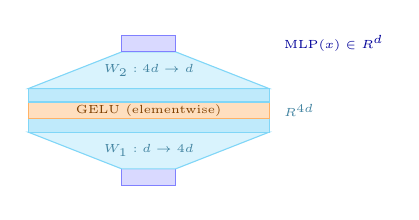
\begin{tikzpicture}[font=\footnotesize, scale=0.85, every node/.style={transform shape}]
        % Input vector (d)
        \node[font=\tiny, text=blue!60!black, anchor=south] at (0, -0.05) {$x \in \mathbb{R}^d$};
        \draw[fill=blue!15, draw=blue!50] (-0.4, 0.05) rectangle (0.4, 0.30);

        % W_1 trapezoid d -> 4d
        \draw[fill=cyan!15, draw=cyan!50]
          (-0.4, 0.30) -- (0.4, 0.30) -- (1.8, 0.85) -- (-1.8, 0.85) -- cycle;
        \node[font=\tiny, text=cyan!60!black] at (0, 0.575) {$W_1: d \to 4d$};

        % 4d wide bar
        \draw[fill=cyan!25, draw=cyan!50] (-1.8, 0.85) rectangle (1.8, 1.05);

        % GELU bar
        \draw[fill=orange!25, draw=orange!60] (-1.8, 1.05) rectangle (1.8, 1.30);
        \node[font=\tiny, text=orange!50!black] at (0, 1.175) {GELU (elementwise)};

        % 4d wide bar after GELU
        \draw[fill=cyan!25, draw=cyan!50] (-1.8, 1.30) rectangle (1.8, 1.50);
        \node[font=\tiny, text=cyan!60!black, anchor=west] at (1.9, 1.175) {$\mathbb{R}^{4d}$};

        % W_2 trapezoid 4d -> d
        \draw[fill=cyan!15, draw=cyan!50]
          (-1.8, 1.50) -- (1.8, 1.50) -- (0.4, 2.05) -- (-0.4, 2.05) -- cycle;
        \node[font=\tiny, text=cyan!60!black] at (0, 1.775) {$W_2: 4d \to d$};

        % output bar
        \draw[fill=blue!15, draw=blue!50] (-0.4, 2.05) rectangle (0.4, 2.30);
        \node[font=\tiny, text=blue!60!black, anchor=west] at (1.9, 2.175) {$\mathrm{MLP}(x) \in \mathbb{R}^d$};
      \end{tikzpicture}
    \end{column}
  \end{columns}

  \vspace{0.2em}
  \begin{columns}
    \begin{column}{0.55\textwidth}
      \textbf{GELU} (Gaussian Error Linear Unit):
      \begin{itemize}
        \itemsep0.15em
        \item $\mathrm{GELU}(x) = x \cdot \Phi(x)$ where $\Phi$ is the standard normal CDF:
          \[
            \Phi(x) = \tfrac{1}{\sqrt{2\pi}} \int_{-\infty}^x e^{-t^2/2}\,dt
                   = \tfrac{1}{2}\!\left[1 + \mathrm{erf}(x/\sqrt{2})\right]
          \]
        \item $\mathrm{erf}(x) = \tfrac{2}{\sqrt{\pi}}\int_0^x e^{-t^2}\,dt$: no closed form, slow on GPUs
        \item Smooth, non-zero on negatives; empirically better than ReLU
      \end{itemize}

      \textbf{GPT-2 tanh approximation} (gap $<10^{-4}$):
      \[
        \mathrm{GELU}(x) \approx \tfrac{x}{2}\!\left[1 + \tanh\!\left(\sqrt{2/\pi}\,(x + 0.044715\, x^3)\right)\right]
      \]
      \begin{itemize}
        \itemsep0.1em
        \item Avoids \texttt{erf}; uses only \texttt{tanh} and a cubic.
        \item GPT-2 / BERT were trained with this form.
        \item PyTorch: \texttt{nn.GELU(approximate='tanh')}; see \href{https://github.com/pytorch/pytorch/issues/39853}{pytorch\#39853}.
      \end{itemize}
    \end{column}
    \begin{column}{0.42\textwidth}
      \begin{tikzpicture}
        \begin{axis}[width=5.5cm, height=4.0cm,
          xlabel={$x$}, ylabel={},
          xmin=-3, xmax=3, ymin=-0.2, ymax=3,
          grid=major, grid style={gray!30},
          legend pos=north west, legend style={font=\tiny},
          tick label style={font=\tiny},
          label style={font=\small},
          xtick={-2,0,2}, ytick={0,1,2}]
          \addplot[blue, thick, domain=-3:3, samples=120]
            {x * 0.5 * (1 + myerf(x/sqrt(2)))};
          \addplot[orange, thick, dashed, domain=-3:3, samples=120]
            {x * 0.5 * (1 + tanh(sqrt(2/pi)*(x + 0.044715*x^3)))};
          \addplot[gray, dotted, thick, domain=-3:3, samples=80]
            {max(0,x)};
          \legend{exact GELU, tanh approx., ReLU}
        \end{axis}
      \end{tikzpicture}

      {\centering\footnotesize
      Exact and tanh approx.\ overlap visually.\par}
    \end{column}
  \end{columns}
\end{frame}

% -----------------------------------------------------------------------
\begin{frame}{Weight Tying \& Initialization}

  \begin{columns}
    \begin{column}{0.50\textwidth}
      \textbf{Weight tying}: the token embedding matrix $W_e$ and the LM head are \emph{shared}:
      \begin{center}
        \texttt{lm\_head.weight = transformer.wte.weight}
      \end{center}
      \begin{itemize}
        \item Saves $V \times d = 50304 \times 768 \approx 38$M parameters
        \item Input and output representations are coupled; works well in practice
      \end{itemize}

      \vspace{0.4em}
      \textbf{Initialization}:
      \begin{itemize}
        \item All weights: $\mathcal{N}(0, 0.02)$, biases: zero
        \item \textbf{Residual projections} (attention \texttt{c\_proj}, MLP \texttt{c\_proj}) scaled by $\frac{0.02}{\sqrt{2L}}$: prevents residual stream variance from growing with depth
      \end{itemize}

      \vspace{0.4em}
      \textbf{Where biases live} (nanoGPT default \texttt{bias=True}, matching original GPT-2):
      \begin{itemize}
        \itemsep0.05em
        \item Linear layers: \texttt{c\_attn}, \texttt{c\_proj} (attn); \texttt{c\_fc}, \texttt{c\_proj} (MLP)
        \item LayerNorm: additive bias $\beta$ (alongside scale $\gamma$)
        \item \emph{Hardcoded \texttt{bias=False}}: \texttt{lm\_head}; embeddings $W_e$, $W_p$ have no bias by construction
      \end{itemize}
      Opt-in \texttt{bias=False} drops all linear biases and LN $\beta$ everywhere: slightly faster and marginally better, but no longer matches OpenAI's released weights.
    \end{column}
    \begin{column}{0.46\textwidth}
      \begin{tikzpicture}[
        box/.style={draw, rounded corners, fill=blue!8, text width=3.2cm, align=center, font=\small, minimum height=0.6cm},
        shared/.style={draw=red!50, rounded corners, fill=red!10, text width=3.2cm, align=center, font=\small, minimum height=0.6cm, line width=0.8pt},
        arr/.style={-Stealth, thick},
      ]
        \node[shared] (tok) at (0,5.2) {Token Embedding $W_e$};
        \node[box] (pos) at (0,4.3) {+ Position Emb.\ $W_p$};
        \node[box] (b1)  at (0,3.4) {Transformer Block $\times 12$};
        \node[box] (ln)  at (0,2.5) {LayerNorm};
        \node[shared] (lm)  at (0,1.6) {LM Head ($= W_e^\top$)};
        \node[box, fill=green!10] (out) at (0,0.7) {Logits over vocab};
        \draw[arr] (tok) -- (pos);
        \draw[arr] (pos) -- (b1);
        \draw[arr] (b1)  -- (ln);
        \draw[arr] (ln)  -- (lm);
        \draw[arr] (lm)  -- (out);

        % Weight tying bracket
        \draw[red!60, thick, dashed, <->, rounded corners=8pt]
          (tok.east) -- ++(0.7, 0) |- (lm.east);
        \node[font=\small, text=red!60, rotate=-90]
          at ([xshift=0.95cm]b1.east) {shared $W_e$};
      \end{tikzpicture}
    \end{column}
  \end{columns}
\end{frame}

\subsection{Optimization}

% -----------------------------------------------------------------------
\begin{frame}{Optimizer: AdamW with Selective Weight Decay}

  \textbf{AdamW} = Adam + decoupled weight decay. Weight decay acts as L2 regularization on the weights directly (not via the gradient).

  \begin{block}{}
    Optimizers (AdamW, Muon, and others) are covered in detail in chapter ``\nameref{ch:optimizers}''.
  \end{block}

  \vspace{0.5em}
  \textbf{Key insight}: not all parameters should be decayed.

  \begin{columns}
    \begin{column}{0.5\textwidth}
      \textbf{Decay} (2D+ tensors):
      \begin{itemize}
        \item Weight matrices in attention ($Q, K, V$, proj)
        \item Weight matrices in MLP
        \item Embedding matrices
      \end{itemize}

      \vspace{0.3em}
      \textbf{No decay} ($<$ 2D tensors):
      \begin{itemize}
        \item Biases
        \item LayerNorm scales (1D)
      \end{itemize}
    \end{column}
    \begin{column}{0.46\textwidth}
      \begin{block}{Why not decay everything?}
        Biases and LayerNorm parameters are scale/shift terms. Penalizing their magnitude does not help as regularization and can harm training.
      \end{block}

      \vspace{0.3em}
      \begin{block}{Fused AdamW}
        PyTorch offers a CUDA-fused implementation that combines the optimizer update into a single kernel, giving a meaningful speedup.
      \end{block}
    \end{column}
  \end{columns}
\end{frame}

% -----------------------------------------------------------------------
\begin{frame}{Learning Rate Schedule: Cosine with Warmup}

  \begin{columns}
    \begin{column}{0.5\textwidth}
      Three-phase schedule:
      \begin{enumerate}
        \item \textbf{Linear warmup} (0 to \texttt{warmup\_iters}):
          \[
            \eta_t = \eta_{\max} \cdot \frac{t+1}{\texttt{warmup\_iters}+1}
          \]
        \item \textbf{Cosine decay} (\texttt{warmup\_iters} to \texttt{lr\_decay\_iters}):
          \[
            \eta_t = \eta_{\min} + \frac{1 + \cos(\pi r)}{2}(\eta_{\max} - \eta_{\min})
          \]
          where $r = \frac{t - \texttt{warmup}}{\texttt{decay} - \texttt{warmup}}$
        \item \textbf{Constant} $\eta_{\min}$ afterwards
      \end{enumerate}
      \vspace{0.3em}
      Follows Chinchilla scaling law recommendations~\cite{hoffmann2022chinchilla}: $\eta_{\min} \approx \eta_{\max}/10$.

      \vspace{0.3em}
      \textbf{Typical \texttt{warmup\_iters}}: 0.5--2\% of total iters. GPT-2 used 2{,}000 of 600{,}000 ($\sim$0.3\%); GPT-3 / LLaMA-style runs use a few thousand iters or roughly 0.5--1\%.
    \end{column}
    \begin{column}{0.46\textwidth}
      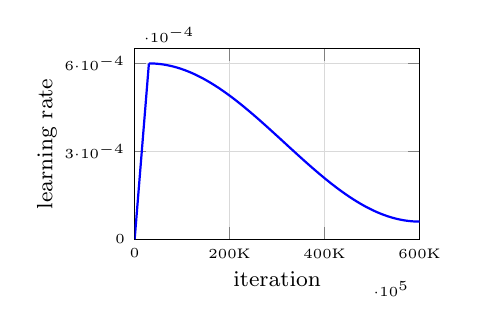
\begin{tikzpicture}
        \begin{axis}[width=5.2cm, height=4.0cm,
          xlabel={iteration}, ylabel={learning rate},
          xmin=0, xmax=600000,
          ymin=0, ymax=0.00065,
          grid=major, grid style={gray!30},
          tick label style={font=\tiny},
          label style={font=\footnotesize},
          xlabel style={yshift=2pt},
          ylabel style={yshift=-4pt},
          xtick={0,200000,400000,600000},
          xticklabels={0,200K,400K,600K},
          ytick={0,0.0003,0.0006},
          yticklabels={0,$3{\cdot}10^{-4}$,$6{\cdot}10^{-4}$},
          ]
          % warmup: 0 to 30000 (exaggerated for visibility; actual GPT-2 used 2000)
          \addplot[blue, thick, domain=0:30000, samples=20]
            {6e-4 * (x+1)/30001};
          % cosine decay: 30000 to 600000
          \addplot[blue, thick, domain=30000:600000, samples=200]
            {6e-5 + 0.5*(1+cos(deg((x-30000)/570000*pi)))*(6e-4-6e-5)};
        \end{axis}
      \end{tikzpicture}
    \end{column}
  \end{columns}
\end{frame}

% -----------------------------------------------------------------------
\begin{frame}{Gradient Accumulation}

  \textbf{Problem}: large effective batch sizes don't fit in GPU memory.

  \vspace{0.5em}
  \textbf{Solution}: accumulate gradients over multiple micro-batches before doing one optimizer step.

  \vspace{0.5em}
  \begin{columns}
    \begin{column}{0.55\textwidth}
      With \texttt{gradient\_accumulation\_steps} $= G$:
      \begin{enumerate}
        \item For $g = 1, \ldots, G$: forward + backward on micro-batch, \emph{accumulate} gradients (no optimizer step)
        \item After $G$ steps: \texttt{optimizer.step()}, then \texttt{zero\_grad()}
      \end{enumerate}

      \vspace{0.4em}
      Mathematically equivalent to training on one big batch of size $G \times B$, since gradients add linearly.

      \vspace{0.3em}
      \textbf{Important}: divide the loss by $G$ before each backward pass to keep the scale consistent:
      \begin{center}
        \texttt{loss = loss / gradient\_accumulation\_steps}
      \end{center}
    \end{column}
    \begin{column}{0.42\textwidth}
      \begin{tikzpicture}[font=\small,
        sbox/.style={draw, fill=blue!10, rounded corners, minimum width=2.8cm, minimum height=0.6cm, align=center},
        arr/.style={-Stealth, thick}]
        \node[sbox] (m1) at (0,4.0) {micro-batch 1: fwd+bwd};
        \node[sbox] (m2) at (0,3.1) {micro-batch 2: fwd+bwd};
        \node[font=\small] at (0,2.4) {$\vdots$};
        \node[sbox] (mG) at (0,1.7) {micro-batch $G$: fwd+bwd};
        \node[sbox, fill=green!15] (opt) at (0,0.7) {optimizer.step()};
        \draw[arr] (m1) -- (m2);
        \draw[arr] (m2) -- ($(m2.south)+(0,-0.3)$);
        \draw[arr] (mG) -- (opt);
        % gradient accumulation brace
        \draw[decorate, decoration={brace, amplitude=5pt}, thick]
          (1.8,4.3) -- (1.8,1.4) node[midway, right=6pt, font=\tiny, align=left] {grad\\accum};
      \end{tikzpicture}
    \end{column}
  \end{columns}
\end{frame}

% -----------------------------------------------------------------------
\begin{frame}{Gradient Clipping}

  \textbf{Problem}: in deep networks, gradients can occasionally explode, destabilizing training.

  \vspace{0.5em}
  \textbf{Solution}: clip the global gradient norm before the optimizer step.

  \[
    \text{if } \|\nabla\|_2 > \texttt{grad\_clip}: \quad \nabla \leftarrow \frac{\texttt{grad\_clip}}{\|\nabla\|_2} \cdot \nabla
  \]

  \begin{columns}
    \begin{column}{0.55\textwidth}
      \begin{itemize}
        \item The global norm is computed over \emph{all} parameters jointly
        \item Only rescales when the norm exceeds the threshold (here: 1.0)
        \item Does not change gradient direction, only magnitude
        \item Applied \emph{after} unscaling (when using GradScaler with float16)
      \end{itemize}
    \end{column}
    \begin{column}{0.42\textwidth}
      \begin{block}{In code}
        \small
        \texttt{scaler.unscale\_(optimizer)} \\
        \texttt{torch.nn.utils.clip\_grad\_norm\_(} \\
        \texttt{\quad model.parameters(), 1.0)} \\
        \texttt{scaler.step(optimizer)}
      \end{block}
      \vspace{0.3em}
      A few large gradient events per training run is normal; frequent clipping suggests a learning rate that is too high.
    \end{column}
  \end{columns}
\end{frame}

\subsection{Mixed Precision Training}

% -----------------------------------------------------------------------
\begin{frame}{Floating Point Formats for Deep Learning}

  IEEE 754 representation: $(-1)^{S} \times 2^{\,E - \mathrm{bias}} \times (1 + \sum_{i=1}^{m} b_i \, 2^{-i})$, \; bias $= 2^{e-1}{-}1$.

  \vspace{0.3em}
  \begin{center}
  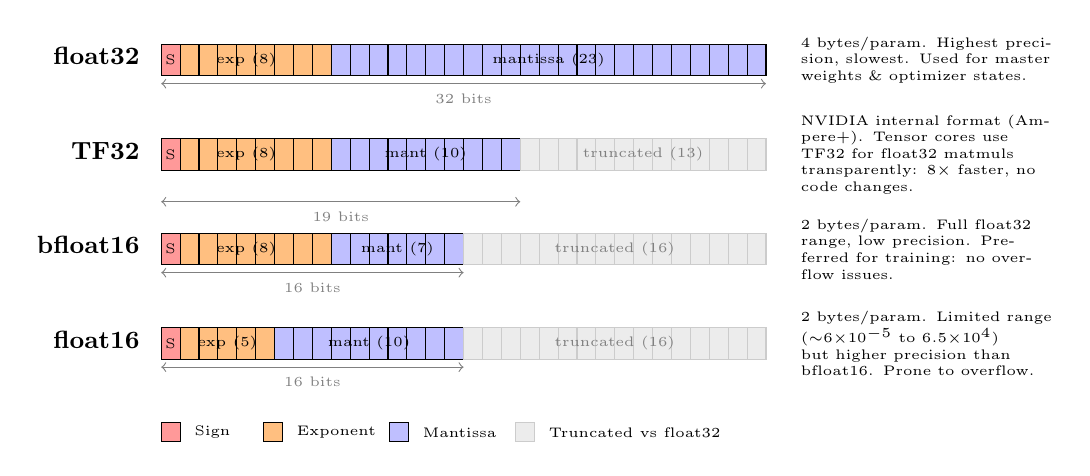
\begin{tikzpicture}[x=1cm, y=1cm]

    % --- float32 (32 bits: 1+8+23) ---
    \node[font=\small\bfseries, anchor=east] at (-0.15, 5.7) {float32};
    \begin{scope}[xshift=0cm, yshift=5.45cm]
      \fill[red!40] (0,0) rectangle (0.24,0.40); \draw (0,0) rectangle (0.24,0.40);
      \node[font=\tiny] at (0.12,0.20) {S};
    \end{scope}
    \begin{scope}[xshift=0.24cm, yshift=5.45cm]
      \foreach \i in {0,...,7} {
        \fill[orange!50] (\i*0.24,0) rectangle (\i*0.24+0.24,0.40);
        \draw (\i*0.24,0) rectangle (\i*0.24+0.24,0.40);
      }
      \node[font=\tiny] at (4*0.24-0.12,0.20) {exp (8)};
    \end{scope}
    \begin{scope}[xshift=2.16cm, yshift=5.45cm]
      \foreach \i in {0,...,22} {
        \fill[blue!25] (\i*0.24,0) rectangle (\i*0.24+0.24,0.40);
        \draw (\i*0.24,0) rectangle (\i*0.24+0.24,0.40);
      }
      \node[font=\tiny] at (11.5*0.24,0.20) {mantissa (23)};
    \end{scope}
    \draw[<->, gray, thin] (0,5.35) -- (32*0.24,5.35) node[midway, below, font=\tiny, gray] {32 bits};
    % annotation
    \node[font=\tiny, anchor=west, align=left, text width=3.2cm] at (8.0, 5.65)
      {4 bytes/param. Highest precision, slowest. Used for master weights \& optimizer states.};

    % --- TF32 (19 bits: 1+8+10) ---
    \node[font=\small\bfseries, anchor=east] at (-0.15, 4.5) {TF32};
    \begin{scope}[xshift=0cm, yshift=4.25cm]
      \fill[red!40] (0,0) rectangle (0.24,0.40); \draw (0,0) rectangle (0.24,0.40);
      \node[font=\tiny] at (0.12,0.20) {S};
    \end{scope}
    \begin{scope}[xshift=0.24cm, yshift=4.25cm]
      \foreach \i in {0,...,7} {
        \fill[orange!50] (\i*0.24,0) rectangle (\i*0.24+0.24,0.40);
        \draw (\i*0.24,0) rectangle (\i*0.24+0.24,0.40);
      }
      \node[font=\tiny] at (4*0.24-0.12,0.20) {exp (8)};
    \end{scope}
    \begin{scope}[xshift=2.16cm, yshift=4.25cm]
      \foreach \i in {0,...,9} {
        \fill[blue!25] (\i*0.24,0) rectangle (\i*0.24+0.24,0.40);
        \draw (\i*0.24,0) rectangle (\i*0.24+0.24,0.40);
      }
      \node[font=\tiny] at (5*0.24,0.20) {mant (10)};
    \end{scope}
    % truncated portion
    \begin{scope}[xshift=4.56cm, yshift=4.25cm]
      \foreach \i in {0,...,12} {
        \fill[gray!15] (\i*0.24,0) rectangle (\i*0.24+0.24,0.40);
        \draw[gray!40] (\i*0.24,0) rectangle (\i*0.24+0.24,0.40);
      }
      \node[font=\tiny, gray] at (6.5*0.24,0.20) {truncated (13)};
    \end{scope}
    \draw[<->, gray, thin] (0,3.85) -- (19*0.24,3.85) node[midway, below, font=\tiny, gray] {19 bits};
    % annotation
    \node[font=\tiny, anchor=west, align=left, text width=3.2cm] at (8.0, 4.45)
      {NVIDIA internal format (Ampere+). Tensor cores use TF32 for float32 matmuls transparently: 8$\times$ faster, no code changes.};

    % --- bfloat16 (16 bits: 1+8+7) ---
    \node[font=\small\bfseries, anchor=east] at (-0.15, 3.3) {bfloat16};
    \begin{scope}[xshift=0cm, yshift=3.05cm]
      \fill[red!40] (0,0) rectangle (0.24,0.40); \draw (0,0) rectangle (0.24,0.40);
      \node[font=\tiny] at (0.12,0.20) {S};
    \end{scope}
    \begin{scope}[xshift=0.24cm, yshift=3.05cm]
      \foreach \i in {0,...,7} {
        \fill[orange!50] (\i*0.24,0) rectangle (\i*0.24+0.24,0.40);
        \draw (\i*0.24,0) rectangle (\i*0.24+0.24,0.40);
      }
      \node[font=\tiny] at (4*0.24-0.12,0.20) {exp (8)};
    \end{scope}
    \begin{scope}[xshift=2.16cm, yshift=3.05cm]
      \foreach \i in {0,...,6} {
        \fill[blue!25] (\i*0.24,0) rectangle (\i*0.24+0.24,0.40);
        \draw (\i*0.24,0) rectangle (\i*0.24+0.24,0.40);
      }
      \node[font=\tiny] at (3.5*0.24,0.20) {mant (7)};
    \end{scope}
    \begin{scope}[xshift=3.84cm, yshift=3.05cm]
      \foreach \i in {0,...,15} {
        \fill[gray!15] (\i*0.24,0) rectangle (\i*0.24+0.24,0.40);
        \draw[gray!40] (\i*0.24,0) rectangle (\i*0.24+0.24,0.40);
      }
      \node[font=\tiny, gray] at (8*0.24,0.20) {truncated (16)};
    \end{scope}
    \draw[<->, gray, thin] (0,2.95) -- (16*0.24,2.95) node[midway, below, font=\tiny, gray] {16 bits};
    % annotation
    \node[font=\tiny, anchor=west, align=left, text width=3.2cm] at (8.0, 3.25)
      {2 bytes/param. Full float32 range, low precision. Preferred for training: no overflow issues.};

    % --- float16 (16 bits: 1+5+10) ---
    \node[font=\small\bfseries, anchor=east] at (-0.15, 2.1) {float16};
    \begin{scope}[xshift=0cm, yshift=1.85cm]
      \fill[red!40] (0,0) rectangle (0.24,0.40); \draw (0,0) rectangle (0.24,0.40);
      \node[font=\tiny] at (0.12,0.20) {S};
    \end{scope}
    \begin{scope}[xshift=0.24cm, yshift=1.85cm]
      \foreach \i in {0,...,4} {
        \fill[orange!50] (\i*0.24,0) rectangle (\i*0.24+0.24,0.40);
        \draw (\i*0.24,0) rectangle (\i*0.24+0.24,0.40);
      }
      \node[font=\tiny] at (2.5*0.24,0.20) {exp (5)};
    \end{scope}
    \begin{scope}[xshift=1.44cm, yshift=1.85cm]
      \foreach \i in {0,...,9} {
        \fill[blue!25] (\i*0.24,0) rectangle (\i*0.24+0.24,0.40);
        \draw (\i*0.24,0) rectangle (\i*0.24+0.24,0.40);
      }
      \node[font=\tiny] at (5*0.24,0.20) {mant (10)};
    \end{scope}
    \begin{scope}[xshift=3.84cm, yshift=1.85cm]
      \foreach \i in {0,...,15} {
        \fill[gray!15] (\i*0.24,0) rectangle (\i*0.24+0.24,0.40);
        \draw[gray!40] (\i*0.24,0) rectangle (\i*0.24+0.24,0.40);
      }
      \node[font=\tiny, gray] at (8*0.24,0.20) {truncated (16)};
    \end{scope}
    \draw[<->, gray, thin] (0,1.75) -- (16*0.24,1.75) node[midway, below, font=\tiny, gray] {16 bits};
    % annotation
    \node[font=\tiny, anchor=west, align=left, text width=3.2cm] at (8.0, 2.05)
      {2 bytes/param. Limited range ($\sim$$6{\times}10^{-5}$ to $6.5{\times}10^4$) but higher precision than bfloat16. Prone to overflow.};

    % legend
    \fill[red!40]    (0.0, 0.8) rectangle (0.24,1.05); \draw (0.0,0.8) rectangle (0.24,1.05);
    \node[font=\tiny, anchor=west] at (0.30, 0.92) {Sign};
    \fill[orange!50] (1.3, 0.8) rectangle (1.54,1.05); \draw (1.3,0.8) rectangle (1.54,1.05);
    \node[font=\tiny, anchor=west] at (1.60, 0.92) {Exponent};
    \fill[blue!25]   (2.9, 0.8) rectangle (3.14,1.05); \draw (2.9,0.8) rectangle (3.14,1.05);
    \node[font=\tiny, anchor=west] at (3.20, 0.92) {Mantissa};
    \fill[gray!15]   (4.5, 0.8) rectangle (4.74,1.05); \draw[gray!40] (4.5,0.8) rectangle (4.74,1.05);
    \node[font=\tiny, anchor=west] at (4.80, 0.92) {Truncated vs float32};

  \end{tikzpicture}
  \end{center}

  \vspace{-0.3em}
  {\small
  \textbf{Key trade-off}: more exponent bits $\Rightarrow$ larger dynamic range; more mantissa bits $\Rightarrow$ higher precision.
  bfloat16 and TF32 keep float32's 8-bit exponent (same range), while float16 trades range for precision.}
\end{frame}

% -----------------------------------------------------------------------
\begin{frame}{Mixed-Precision Matrix Multiplication}

  Given $A \in \mathbb{R}^{m \times n}$, $B \in \mathbb{R}^{n \times p}$, compute $C = A \cdot B$ where $C_{ij} = \sum_{k=1}^{n} A_{ik} \cdot B_{kj}$.

  \vspace{0.3em}
  \textbf{Mixed-precision approach}: store and multiply in low precision, accumulate in high precision:
  \[
    C_{ij} = \underbrace{\sum_{k=1}^{n}
      \overbrace{\mathrm{bf16}(A_{ik})}^{\text{cast to bf16}} \cdot
      \overbrace{\mathrm{bf16}(B_{kj})}^{\text{cast to bf16}}
    }_{\text{accumulated in float32}}
    \quad \in \text{float32}
  \]

  \vspace{0.3em}
  \begin{columns}
    \begin{column}{0.48\textwidth}
      \textbf{Step by step}:
      \begin{enumerate}
        \item Cast $A$, $B$ from float32 to bfloat16
        \item Each product $A_{ik} \cdot B_{kj}$: bf16 $\times$ bf16
        \item Running sum $C_{ij} \mathrel{+}= \ldots$ kept in float32
        \item Result $C$ is in float32
      \end{enumerate}

      \vspace{0.3em}
      \textbf{Why not accumulate in bf16?}

      With $n = 768$, summing 768 small products in bf16 (7-bit mantissa $\approx$ 2 decimal digits) leads to severe rounding error. Float32 (23-bit mantissa) preserves accuracy.
    \end{column}
    \begin{column}{0.48\textwidth}
      \textbf{Speedup sources}:
      \begin{itemize}
        \item bf16 values are 2$\times$ smaller $\Rightarrow$ 2$\times$ less memory bandwidth
        \item Tensor cores process bf16 at 2--8$\times$ the float32 throughput
        \item Float32 accumulation is ``free'', built into the tensor core hardware
      \end{itemize}

      \vspace{0.3em}
      \begin{block}{In PyTorch}
        \texttt{torch.amp.autocast} automatically casts matmul inputs to bf16 while the accumulator stays in float32. No manual casting needed.
      \end{block}
    \end{column}
  \end{columns}

\end{frame}

% -----------------------------------------------------------------------
\begin{frame}{Mixed Precision Training}

  \textbf{Goal}: reduced-precision floats save memory and speed up computation, while keeping full precision where it matters.

  \begin{center}
  \begin{tikzpicture}[font=\small, scale=0.68, every node/.style={transform shape},
    box/.style={draw, thick, rounded corners=3pt, minimum width=2.6cm, minimum height=0.6cm, align=center},
    fp32/.style={box, fill=violet!15},
    bf16/.style={box, fill=green!15},
    op/.style={box, fill=blue!10, font=\small\bfseries},
    cast/.style={box, fill=orange!15, font=\small},
    arr/.style={-Stealth, thick},
    lbl/.style={font=\tiny, gray, align=center},
  ]
    % === Left: Storage ===
    \node[fp32] (mw) at (0, 7.02) {Master weights $\theta$};
    \node[lbl, above=0pt of mw] {float32};

    % Cast down
    \node[cast] (castdown) at (0, 5.85) {cast to bf16};
    \draw[arr] (mw) -- (castdown);

    % bf16 weights copy
    \node[bf16] (wbf) at (0, 4.68) {Weights $\hat{\theta}$};
    \node[lbl, right=2pt of wbf] {bfloat16};
    \draw[arr] (castdown) -- (wbf);

    % Forward
    \node[op] (fwd) at (0, 3.51) {Forward pass};
    \node[lbl, above right=1pt and 2pt of fwd] {bf16 compute};
    \draw[arr] (wbf) -- (fwd);

    % Input
    \node[bf16, minimum width=1.8cm] (input) at (-3.5, 3.51) {Input $x$};
    \node[lbl, above=0pt of input] {bf16};
    \draw[arr] (input) -- (fwd);

    % Loss (fp32)
    \node[fp32, minimum width=1.8cm] (loss) at (3.5, 3.51) {Loss $\mathcal{L}$};
    \node[lbl, above=0pt of loss] {float32};
    \draw[arr] (fwd) -- (loss);

    % Activations stored
    \node[bf16, minimum width=1.8cm] (act) at (-3.5, 2.34) {Activations};
    \node[lbl, above=0pt of act] {bf16};
    \draw[arr, dashed, green!50!black] (fwd) -- (act);

    % Backward
    \node[op] (bwd) at (0, 2.34) {Backward pass};
    \node[lbl, above=0pt of bwd] {bf16 compute};
    \draw[arr] (loss) |- (bwd);
    \draw[arr, dashed, green!50!black] (act) -- (bwd);

    % Gradients in fp32
    \node[fp32] (grad) at (0, 1.17) {Gradients $\nabla_\theta \mathcal{L}$};
    \node[lbl, right=2pt of grad] {float32};
    \draw[arr] (bwd) -- (grad);

    % Optimizer
    \node[op] (opt) at (0, 0.0) {Optimizer step (AdamW)};
    \draw[arr] (grad) -- (opt);

    % Optimizer states
    \node[fp32, minimum width=2.2cm] (states) at (-3.5, 0.0) {$m_t, v_t$};
    \node[lbl, above=0pt of states] {float32};
    \draw[arr, <->] (states) -- (opt);

    % Update master weights
    \draw[arr] (opt.east) -- ++(1.0,0) node[lbl, right] {$\theta \leftarrow \theta - \eta \cdot \text{update}$} -- ++(2.0,0) |- (mw.east);

    % Legend at bottom
    \node[fp32, minimum width=1.0cm, minimum height=0.35cm, font=\tiny] at (-3.5, -1.105) {float32};
    \node[bf16, minimum width=1.0cm, minimum height=0.35cm, font=\tiny] at (-1.8, -1.105) {bfloat16};
    \node[op, minimum width=1.0cm, minimum height=0.35cm, font=\tiny] at (0.0, -1.105) {operation};
    \node[cast, minimum width=1.0cm, minimum height=0.35cm, font=\tiny] at (1.8, -1.105) {cast};

  \end{tikzpicture}
  \end{center}
\end{frame}

% -----------------------------------------------------------------------
\begin{frame}{GradScaler: Handling float16 Underflow}

  \textbf{Problem}: float16 has a small dynamic range ($\approx 6 \times 10^{-5}$ to $6.5 \times 10^4$). Gradients during training are often tiny and \textbf{underflow to zero}.

  \vspace{0.5em}
  \begin{columns}
    \begin{column}{0.52\textwidth}
      \textbf{Solution: loss scaling.}
      \begin{enumerate}
        \item Multiply loss by a large scale factor $S$ before \texttt{backward()}
          \[ \tilde{\mathcal{L}} = S \cdot \mathcal{L} \]
        \item Gradients are also scaled by $S$ (by chain rule)
        \item Before optimizer step: divide gradients by $S$
        \item Check for \texttt{inf}/\texttt{nan}:
          \begin{itemize}
            \item If found: \textbf{skip} the optimizer step, reduce $S$
            \item Otherwise: proceed, slowly increase $S$
          \end{itemize}
      \end{enumerate}

      \vspace{0.3em}
      Not needed for \texttt{bfloat16} (same range as float32).
    \end{column}
    \begin{column}{0.44\textwidth}
      \begin{tikzpicture}[font=\small, scale=0.82, every node/.style={transform shape},
        sbox/.style={draw, rounded corners, fill=blue!8, text width=3.0cm, align=center, minimum height=0.6cm},
        obox/.style={draw, rounded corners, fill=orange!15, text width=3.0cm, align=center, minimum height=0.6cm},
        gbox/.style={draw, rounded corners, fill=green!15, text width=3.0cm, align=center, minimum height=0.6cm},
        arr/.style={-Stealth, thick}]
        \node[sbox] (loss)  at (0, 5.0) {loss $\mathcal{L}$};
        \node[obox] (scale) at (0, 4.0) {$\times\, S$ (scale up)};
        \node[sbox] (bwd)   at (0, 3.0) {backward()};
        \node[obox] (unsc)  at (0, 2.0) {$\div\, S$ (unscale)};
        \node[sbox] (clip)  at (0, 1.0) {grad clip};
        \node[gbox] (opt)   at (0, 0.0) {optimizer.step()};
        \draw[arr] (loss)  -- (scale);
        \draw[arr] (scale) -- (bwd);
        \draw[arr] (bwd)   -- (unsc);
        \draw[arr] (unsc)  -- (clip);
        \draw[arr] (clip)  -- (opt);
        % inf/nan branch: skip clip + step, reduce S
        \node[font=\tiny, red, align=center] (skip) at (3.4, 0.5) {inf/nan?\\skip step\\reduce $S$};
        \draw[-Stealth, red, dashed, thick]
          (unsc.east) -| (skip.north);
      \end{tikzpicture}
    \end{column}
  \end{columns}
\end{frame}

% -----------------------------------------------------------------------

\subsection{Compilation and Kernel Fusion}

% -----------------------------------------------------------------------
\begin{frame}{\texttt{torch.compile}}

  PyTorch 2.0 introduced \texttt{torch.compile(model)}, which JIT-compiles the model graph.

  \vspace{0.5em}
  \begin{columns}
    \begin{column}{0.55\textwidth}
      \textbf{How it works}:
      \begin{enumerate}
        \item \textbf{TorchDynamo}: captures the computation graph by tracing Python bytecode
        \item \textbf{TorchInductor}: backend compiler that generates optimized Triton (GPU) or C++ (CPU) code
      \end{enumerate}

      \vspace{0.4em}
      \textbf{What it optimizes}:
      \begin{itemize}
        \item \textbf{Kernel fusion}: merges adjacent operations into one kernel (e.g., LayerNorm + dropout), reducing memory bandwidth
        \item \textbf{Memory layout}: reorders ops to maximize cache reuse
        \item Eliminates Python overhead in the hot path
      \end{itemize}
    \end{column}
    \begin{column}{0.42\textwidth}
      \begin{alertblock}{Cost}
        First forward pass triggers compilation (takes $\sim$1 minute). Subsequent passes use the cached compiled graph.
      \end{alertblock}

      \vspace{0.5em}
      \begin{block}{Typical speedup}
        15--30\% throughput improvement for GPT-2 scale models.
      \end{block}
    \end{column}
  \end{columns}
\end{frame}

% -----------------------------------------------------------------------
\begin{frame}{Kernel Fusion: Softmax + Cross-Entropy (Forward)}

  Given logits $z \in \mathbb{R}^V$ and target class $y$:
  \[
    p_i = \frac{e^{z_i}}{\sum_{j} e^{z_j}} \quad \text{(softmax)}, \qquad
    \mathcal{L} = -\log p_y \;=\; -z_y + \log \sum_{j} e^{z_j} \quad \text{(cross-entropy)}
  \]

  \vspace{-0.5em}
  \begin{columns}
    \begin{column}{0.48\textwidth}
      \centering\textbf{Unfused: 3 kernel launches}

      \vspace{0.2em}
      \begin{tikzpicture}[scale=0.78, every node/.style={transform shape},
        stp/.style={draw, rounded corners=2pt, fill=blue!8, font=\small,
                    minimum width=3.0cm, minimum height=0.45cm, align=center},
        hbm/.style={draw, rounded corners=2pt, fill=red!8, font=\tiny,
                    minimum width=3.0cm, minimum height=0.35cm, align=center},
        inp/.style={draw, rounded corners=2pt, fill=gray!12, font=\tiny,
                    minimum width=3.0cm, minimum height=0.35cm, align=center},
        arr/.style={-Stealth, thick},
      ]
        \node[inp] (z)    at (0, 7.0) {logits $z \in \mathbb{R}^V$ \quad{\tiny (in GPU memory)}};

        % Kernel 1: softmax
        \node[stp] (k1s1) at (0, 6.3) {$p_i = e^{z_i} / \sum_j e^{z_j}$};
        \node[hbm] (k1o)  at (0, 5.6) {write $p$ to GPU memory};
        \node[draw=red!60, dashed, rounded corners=3pt, inner sep=3pt,
              fit=(k1s1)(k1o), label={[font=\tiny\bfseries, red!70]right:Kernel 1}] {};

        % GPU memory read
        \node[hbm] (r1)   at (0, 4.9) {read $p$ from GPU memory};

        % Kernel 2: log
        \node[stp] (k2s1) at (0, 4.2) {$\ell_i = \log p_i$};
        \node[hbm] (k2o)  at (0, 3.5) {write $\log p$ to GPU memory};
        \node[draw=red!60, dashed, rounded corners=3pt, inner sep=3pt,
              fit=(k2s1)(k2o), label={[font=\tiny\bfseries, red!70]right:Kernel 2}] {};

        % GPU memory read
        \node[hbm] (r2)   at (0, 2.8) {read $\log p$ from GPU memory};

        % Kernel 3: index + negate
        \node[stp] (k3s1) at (0, 2.1) {$\mathcal{L} = -\ell_y$};
        \node[draw=red!60, dashed, rounded corners=3pt, inner sep=3pt,
              fit=(k3s1), label={[font=\tiny\bfseries, red!70]right:Kernel 3}] {};

        \node[inp] (L)    at (0, 1.4) {loss $\mathcal{L}$};

        \draw[arr]        (z)    -- (k1s1);
        \draw[arr]        (k1s1) -- (k1o);
        \draw[arr, red!50] (k1o)  -- (r1);
        \draw[arr]        (r1)   -- (k2s1);
        \draw[arr]        (k2s1) -- (k2o);
        \draw[arr, red!50] (k2o)  -- (r2);
        \draw[arr]        (r2)   -- (k3s1);
        \draw[arr]        (k3s1) -- (L);
      \end{tikzpicture}

      \vspace{0.3em}
      \begin{itemize}\footnotesize
        \itemsep0.1em
        \item \textcolor{red!70}{\textbf{Each kernel}}: read from memory, compute, write back.
      \end{itemize}
    \end{column}
    \begin{column}{0.48\textwidth}
      \centering\textbf{Fused: 1 kernel launch}

      \vspace{0.2em}
      \begin{tikzpicture}[scale=0.78, every node/.style={transform shape},
        inp/.style={rectangle, draw=gray!60, fill=gray!12, rounded corners=2pt, font=\tiny,
                    minimum width=2.6cm, minimum height=0.35cm},
        fused/.style={rectangle, draw=green!60!black, fill=green!10, rounded corners=4pt, font=\small,
                      minimum width=2.6cm, align=center},
        reg/.style={rectangle, draw=blue!40, fill=blue!6, rounded corners=2pt, font=\tiny,
                    minimum width=2.2cm, minimum height=0.3cm, align=center},
        arr/.style={-Stealth, thick},
      ]
        \node[inp] (z)  at (0, 7.0) {logits $z \in \mathbb{R}^V$};

        \node[fused, minimum height=2.6cm, text width=2.4cm] (fk) at (0, 4.8) {};
        % internal steps as small labels inside the box
        \node[reg] at (0, 5.4) {$m = \max(z)$};
        \node[reg] at (0, 4.8) {$s = \sum e^{z_i - m}$};
        \node[reg] at (0, 4.2) {$\mathcal{L} = {-}z_y {+} m {+} \log s$};

        \node[inp] (L) at (0, 2.6) {loss $\mathcal{L}$};

        \draw[arr] (z)  -- (fk);
        \draw[arr] (fk) -- (L);
      \end{tikzpicture}

      \vspace{0.3em}
      \begin{itemize}\footnotesize
        \itemsep0.1em
        \item \textcolor{green!60!black}{\textbf{No GPU memory writes}} of $e^z$, $p$, $\log p$: all computed in registers.
        \item Cross-entropy computed directly from logits, no need to materialise $p$.
      \end{itemize}
    \end{column}
  \end{columns}
\end{frame}

% -----------------------------------------------------------------------
\begin{frame}{Kernel Fusion: Softmax + Cross-Entropy (Backward)}

  Gradient of cross-entropy w.r.t.\ logits:
  \[
    \frac{\partial \mathcal{L}}{\partial z_i} = p_i - \mathbf{1}[i = y], \qquad p = \mathrm{softmax}(z)
  \]

  \vspace{0.3em}
  \begin{columns}
    \begin{column}{0.48\textwidth}
      \centering\textbf{Unfused backward}

      \vspace{0.3em}
      \begin{tikzpicture}[
        op/.style={rectangle, draw=blue!60, fill=blue!10, rounded corners=2pt, font=\tiny,
                   minimum width=2.4cm, minimum height=0.38cm, align=center},
        buf/.style={rectangle, draw=red!50, fill=red!8, rounded corners=2pt, font=\tiny,
                    minimum width=2.4cm, minimum height=0.38cm, align=center},
        inp/.style={rectangle, draw=gray!60, fill=gray!12, rounded corners=2pt, font=\tiny,
                    minimum width=2.4cm, minimum height=0.38cm},
        arr/.style={-Stealth, thick},
        rd/.style={-Stealth, dashed, red!60},
      ]
        \node[inp] (dL)  at (0, 5.2) {$\partial\mathcal{L}/\partial\mathcal{L} = 1$};

        \node[op]  (dnl) at (0, 4.5) {$\nabla[\cdot]_y$};
        \node[buf] (lp)  at (0, 3.8) {$\log p$ \quad\textcolor{red!70}{\textbf{read GPU memory}}};
        \node[op]  (dlg) at (0, 3.1) {$\nabla\log$};
        \node[buf] (p)   at (0, 2.4) {$p$ \quad\textcolor{red!70}{\textbf{read GPU memory}}};
        \node[op]  (dsm) at (0, 1.7) {$\nabla\mathrm{softmax}$};
        \node[buf] (ez)  at (0, 1.0) {$e^z$ \quad\textcolor{red!70}{\textbf{read GPU memory}}};
        \node[inp] (dz)  at (0, 0.3) {$\partial\mathcal{L}/\partial z$};

        \draw[arr] (dL)  -- (dnl);
        \draw[arr] (dnl) -- (lp);
        \draw[arr] (lp)  -- (dlg);
        \draw[arr] (dlg) -- (p);
        \draw[arr] (p)   -- (dsm);
        \draw[arr] (dsm) -- (ez);
        \draw[arr] (ez)  -- (dz);

        \node[font=\tiny, red!60, anchor=west] at (1.35, 3.8) {\#1};
        \node[font=\tiny, red!60, anchor=west] at (1.35, 2.4) {\#2};
        \node[font=\tiny, red!60, anchor=west] at (1.35, 1.0) {\#3};
      \end{tikzpicture}
    \end{column}
    \begin{column}{0.48\textwidth}
      \centering\textbf{Fused backward}

      \vspace{0.3em}
      \begin{tikzpicture}[
        inp/.style={rectangle, draw=gray!60, fill=gray!12, rounded corners=2pt, font=\tiny,
                    minimum width=3.0cm, minimum height=0.38cm},
        fused/.style={rectangle, draw=green!60!black, fill=green!10, rounded corners=4pt, font=\small,
                      minimum width=3.0cm, align=center},
        reg/.style={rectangle, draw=blue!40, fill=blue!6, rounded corners=2pt, font=\tiny,
                    minimum width=2.2cm, minimum height=0.34cm, align=center},
        arr/.style={-Stealth, thick},
      ]
        \node[inp] (z)   at (0, 5.2) {logits $z$ \quad\textcolor{green!60!black}{\textbf{read GPU memory}}};

        \node[fused, minimum height=2.0cm, text width=2.4cm] (fk) at (0, 3.5) {
          \textbf{Fused kernel}
        };
        \node[reg] at (0, 3.9) {recompute $p = \mathrm{softmax}(z)$};
        \node[reg] at (0, 3.1) {$\partial\mathcal{L}/\partial z_i = p_i - \mathbf{1}[i{=}y]$};

        \node[inp] (dz)  at (0, 1.8) {$\partial\mathcal{L}/\partial z$ \quad\textcolor{green!60!black}{\textbf{write GPU memory}}};

        \draw[arr] (z)  -- (fk);
        \draw[arr] (fk) -- (dz);
      \end{tikzpicture}

      \vspace{0.3em}
      \begin{itemize}\footnotesize
        \itemsep0.1em
        \item \textcolor{green!60!black}{\textbf{Only 1 read + 1 write}}: $p$ recomputed in registers, no stored intermediates needed.
      \end{itemize}
    \end{column}
  \end{columns}
\end{frame}

\subsection{Distributed Training and Data Loading}

% -----------------------------------------------------------------------
\begin{frame}{Data Parallelism}

  \begin{columns}[T]
    \begin{column}{0.34\textwidth}
      \textbf{Idea}: replicate the model on every GPU, split the batch.
      \begin{itemize}
        \item Same parameters $\theta$ on each GPU
        \item Each GPU sees a different batch shard
        \item Gradients synced across GPUs after backward
        \item Throughput scales near-linearly with \#GPUs
      \end{itemize}
    \end{column}
    \begin{column}{0.62\textwidth}
      \begin{center}
      \begin{tikzpicture}[font=\footnotesize, scale=0.7, every node/.style={transform shape},
        master/.style={draw, fill=violet!22, rounded corners=2pt, minimum width=2.6cm, minimum height=0.55cm, align=center},
        replica/.style={draw, fill=violet!18, rounded corners=2pt, minimum width=1.6cm, minimum height=0.55cm, align=center},
        batch/.style={draw, fill=orange!28, rounded corners=2pt, minimum width=1.4cm, minimum height=0.55cm, align=center},
        gpu/.style={draw, fill=green!28, rounded corners=2pt, minimum width=1.4cm, minimum height=0.55cm, align=center},
        sync/.style={draw, fill=red!12, circle, minimum size=0.75cm, align=center, font=\scriptsize\bfseries},
        datasplit/.style={draw, dashed, fill=yellow!22, rounded corners=3pt, minimum width=9.8cm, minimum height=0.55cm, align=center},
        arr/.style={-Stealth, semithick},
        syncarr/.style={-Stealth, thick, dashed, teal!70!black},
        netline/.style={red, very thick}
      ]
        % Per-column gray containers (Replica + Batch + GPU)
        \foreach \x in {-4.2, -1.4, 1.4, 4.2} {
          \fill[gray!8, rounded corners=2pt] (\x-0.95, 0.55) rectangle (\x+0.95, 3.95);
          \draw[gray!45, rounded corners=2pt] (\x-0.95, 0.55) rectangle (\x+0.95, 3.95);
        }

        % Data Split
        \node[datasplit] (split) at (0, 5.7) {Data Split};

        % Master copy
        \node[master] (master) at (0, 4.7) {Model (Master Copy)};

        % Brackets from Data Split corners to Master Copy
        \draw[thick] (split.south west) -- ++(0,-0.18);
        \draw[thick] (split.south east) -- ++(0,-0.18);
        \draw[arr, thick] ($(split.south west)+(0,-0.18)$) -- (master.north west);
        \draw[arr, thick] ($(split.south east)+(0,-0.18)$) -- (master.north east);

        % Replicas
        \node[replica] (r1) at (-4.2, 3.5) {Model Replica};
        \node[replica] (r2) at (-1.4, 3.5) {Model Replica};
        \node[replica] (r3) at (1.4, 3.5) {Model Replica};
        \node[replica] (r4) at (4.2, 3.5) {Model Replica};

        % Master to replicas (fan out)
        \draw[arr] (master.south) -- (r1.north);
        \draw[arr] (master.south) -- (r2.north);
        \draw[arr] (master.south) -- (r3.north);
        \draw[arr] (master.south) -- (r4.north);

        % Batches
        \node[batch] (b1) at (-4.2, 2.4) {Batch 1};
        \node[batch] (b2) at (-1.4, 2.4) {Batch 2};
        \node[batch] (b3) at (1.4, 2.4) {Batch 3};
        \node[batch] (b4) at (4.2, 2.4) {Batch 4};

        % Replica to Batch
        \draw[arr] (r1.south) -- (b1.north);
        \draw[arr] (r2.south) -- (b2.north);
        \draw[arr] (r3.south) -- (b3.north);
        \draw[arr] (r4.south) -- (b4.north);

        % Sync circle (between batch 2 and 3, at batch row level)
        \node[sync] (sync) at (0, 2.4) {Sync};
        \node[font=\tiny, gray, below=1pt of sync] {Gradient Sync};

        % Sync to replicas (dashed teal arrows going up)
        \draw[syncarr] (sync.north) -- (r1.south east);
        \draw[syncarr] (sync.north) -- (r2.south);
        \draw[syncarr] (sync.north) -- (r3.south);
        \draw[syncarr] (sync.north) -- (r4.south west);

        % GPUs
        \node[gpu] (g1) at (-4.2, 1.3) {GPU 1};
        \node[gpu] (g2) at (-1.4, 1.3) {GPU 2};
        \node[gpu] (g3) at (1.4, 1.3) {GPU 3};
        \node[gpu] (g4) at (4.2, 1.3) {GPU 4};

        % Batch to GPU
        \draw[arr] (b1.south) -- (g1.north);
        \draw[arr] (b2.south) -- (g2.north);
        \draw[arr] (b3.south) -- (g3.north);
        \draw[arr] (b4.south) -- (g4.north);

        % Red network lines (NCCL ring)
        \draw[netline] (g1.south) -- (-4.2, 0.35);
        \draw[netline] (g2.south) -- (-1.4, 0.35);
        \draw[netline] (g3.south) -- (1.4, 0.35);
        \draw[netline] (g4.south) -- (4.2, 0.35);
        \draw[netline] (-4.2, 0.35) -- (4.2, 0.35);
        \draw[netline] (sync.south) -- (0, 0.35);
      \end{tikzpicture}
      \end{center}
    \end{column}
  \end{columns}
\end{frame}

% -----------------------------------------------------------------------
\begin{frame}{Distributed Data Parallel (DDP)}

  \begin{columns}[T]
    \begin{column}{0.40\textwidth}
      \begin{algorithm}[H]
        \caption{DDP step with gradient accumulation (GPU $i$)}
        \small
        \DontPrintSemicolon
        $\nabla_i \leftarrow 0$\;
        \For{$g = 1, \ldots, G$}{
          $\mathcal{B}_i^{(g)} \leftarrow$ micro-batch shard\;
          $\hat{y} \leftarrow \texttt{forward}(\theta, \mathcal{B}_i^{(g)})$\;
          $\mathcal{L} \leftarrow \tfrac{1}{G}\,\texttt{loss}(\hat{y}, y)$\;
          \eIf{$g = G$}{
            $\nabla_i \mathrel{+}= \texttt{backward}(\mathcal{L})$ \tcp*{sync}
            $\bar{\nabla} \leftarrow \textsc{AllReduce}(\nabla_i)$\;
          }{
            $\nabla_i \mathrel{+}= \texttt{backward}(\mathcal{L})$ \tcp*{no sync}
          }
        }
        $\theta \leftarrow \texttt{optimizer.step}(\theta, \bar{\nabla})$\;
      \end{algorithm}

      \vspace{0.3em}
      \begin{itemize}
        \item Sync only on last micro-step: $G \times$ less communication
        \item Replicas stay bit-identical after the step
      \end{itemize}
    \end{column}
    \begin{column}{0.58\textwidth}
      \begin{tikzpicture}[font=\small, scale=0.75, every node/.style={transform shape},
        gpu/.style={draw, fill=orange!15, rounded corners, minimum width=1.7cm, minimum height=0.7cm, align=center},
        model/.style={draw, fill=blue!8, rounded corners, minimum width=1.7cm, minimum height=0.5cm, align=center, font=\tiny},
        sync/.style={draw, fill=green!15, rounded corners, minimum width=8.0cm, minimum height=0.6cm, align=center},
        arr/.style={-Stealth, thick},
      ]
        % GPU 0
        \node[gpu]        (g0)    at (0, 7.0) {GPU 0};
        \node[model]      (m0)    at (0, 5.6) {model + $\mathcal{B}_0$};
        \node[font=\tiny] (grad0) at (0, 4.2) {$\nabla_0$};
        \draw[arr] (g0) -- (m0);
        \draw[arr] (m0) -- (grad0);

        % GPU 1
        \node[gpu]        (g1)    at (3.0, 7.0) {GPU 1};
        \node[model]      (m1)    at (3.0, 5.6) {model + $\mathcal{B}_1$};
        \node[font=\tiny] (grad1) at (3.0, 4.2) {$\nabla_1$};
        \draw[arr] (g1) -- (m1);
        \draw[arr] (m1) -- (grad1);

        % GPU k
        \node[gpu]        (gk)    at (6.0, 7.0) {GPU $k$};
        \node[model]      (mk)    at (6.0, 5.6) {model + $\mathcal{B}_k$};
        \node[font=\tiny] (gradk) at (6.0, 4.2) {$\nabla_k$};
        \draw[arr] (gk) -- (mk);
        \draw[arr] (mk) -- (gradk);

        % dots between GPU 1 and GPU k
        \node[font=\small] at (4.5, 7.0) {$\cdots$};
        \node[font=\small] at (4.5, 5.6) {$\cdots$};
        \node[font=\small] at (4.5, 4.2) {$\cdots$};

        % All-reduce bar (spans all model nodes)
        \node[sync] (ar) at (3.0, 2.8) {\textbf{all-reduce}: $\bar{\nabla} = \frac{1}{k}\sum_i \nabla_i$};
        \draw[arr] (grad0.south) -- (ar.north -| grad0);
        \draw[arr] (grad1.south) -- (ar.north -| grad1);
        \draw[arr] (gradk.south) -- (ar.north -| gradk);

        % Update
        \node[sync, fill=violet!10] (upd) at (3.0, 1.4) {each GPU: $\theta \leftarrow \theta - \eta \cdot \bar{\nabla}$};
        \draw[arr] (ar) -- (upd);

        % Loop back
        \draw[arr, dashed, gray] (upd.south) -- ++(0,-0.4) -| (-1.2, 7.0) -- (g0.west);
      \end{tikzpicture}
    \end{column}
  \end{columns}
\end{frame}


\subsection{Hyperparameters}

% -----------------------------------------------------------------------
\begin{frame}{Hyperparameters}

  \begin{center}
  \begin{tabular}{lll}
    \toprule
    \textbf{Category} & \textbf{Parameter} & \textbf{Value} \\
    \midrule
    Model     & \texttt{n\_layer}        & 12 \\
              & \texttt{n\_head}         & 12 \\
              & \texttt{n\_embd}         & 768 \\
              & \texttt{block\_size}     & 1024 tokens \\
              & \texttt{vocab\_size}     & 50304 (50257 rounded to $\times$64) \\
              & \texttt{bias}            & False \\
    \midrule
    Optimizer & \texttt{learning\_rate}  & $6 \times 10^{-4}$ \\
              & \texttt{weight\_decay}   & $0.1$ \\
              & $(\beta_1, \beta_2)$     & $(0.9, 0.95)$ \\
              & \texttt{grad\_clip}      & 1.0 \\
    \midrule
    Schedule  & \texttt{warmup\_iters}   & 2000 \\
              & \texttt{lr\_decay\_iters}& 600000 \\
              & \texttt{min\_lr}         & $6 \times 10^{-5}$ ($= \frac{\text{lr}}{10}$) \\
    \midrule
    Batch     & \texttt{batch\_size}     & $\approx 491$K tokens ($= 480 \times 1024$) \\
    \bottomrule
  \end{tabular}
  \end{center}

  Vocabulary size rounded up to a multiple of 64 for GPU efficiency (better utilization of tensor cores).
\end{frame}
